\begin{surferPage}[216 Singularités]{Surfaces avec beaucoup de singularités réelles}
    Comme vu précédemment, la valeur exacte de $\mu(7)$, le plus grand nombre possible
    de singularités sur une surface de degré $7$, est inconnu.
    Nous connaissons seulement une borne supérieure et une borne inférieure : $99\le \mu(7) \le 104$. 


    Il n'est pas surprenant que l'on puisse dire moins de choses encore pour un degré $d$ général.

    Sonja Breske, Oliver Labs et Duco van~Straten furent au moins capables d'adapter
    une construction de S.V.\ Chmutov telle que le nombre maximal connu
    de singularités est également atteint par des surfaces à 
    singularités réelles. 
    \`A ce jour, nous savons :
    \[0,41\bar{6}d^3 \lessapprox \mu(d) \lessapprox 0.44\bar{4} d^3.\]
     D'après ce qui précède, on peut voir la symétrie de la construction et le lien avec 
    le nombre maximal de cellules noires dans l'arrangement de droites :
    \begin{center}
      \begin{tabular}{c@{\qquad}c}
        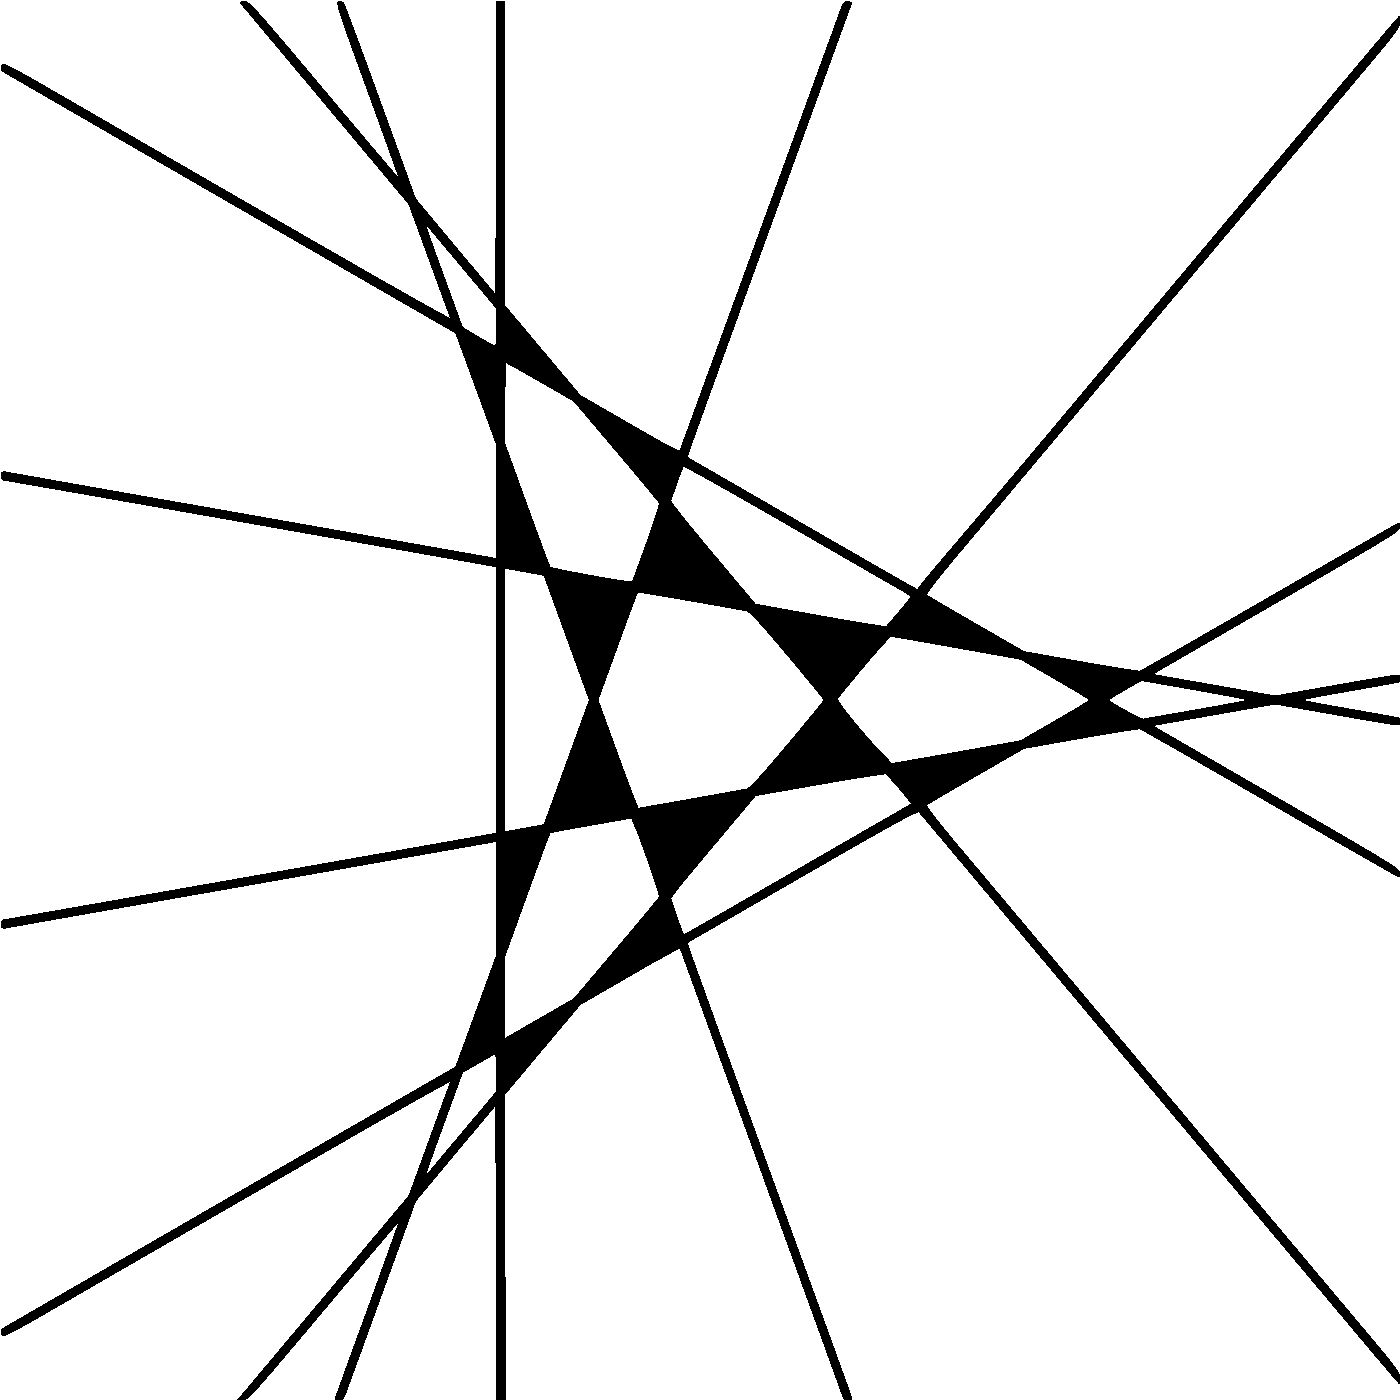
\includegraphics[height=1.5cm]{vielesing.pdf}
        &
        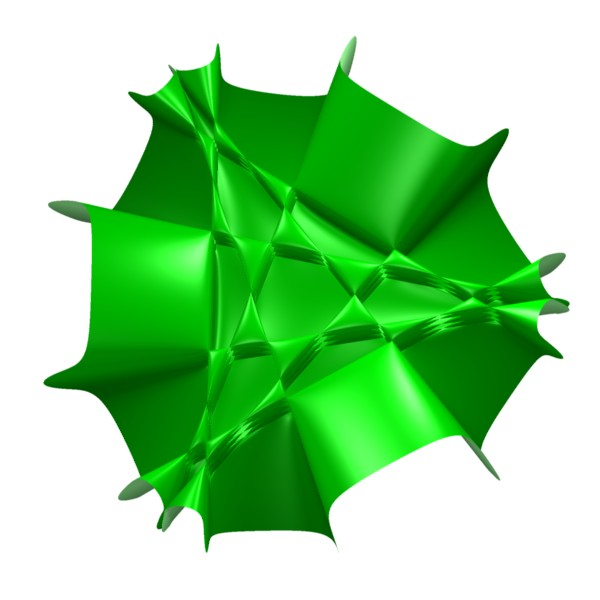
\includegraphics[height=1.5cm]{p9surface_von_oben}
      \end{tabular}
    \end{center}
\end{surferPage}
